\documentclass[tikz,border=8pt]{standalone}
\usepackage[OT4,plmath]{polski}
\usepackage{amsmath}
\begin{document}
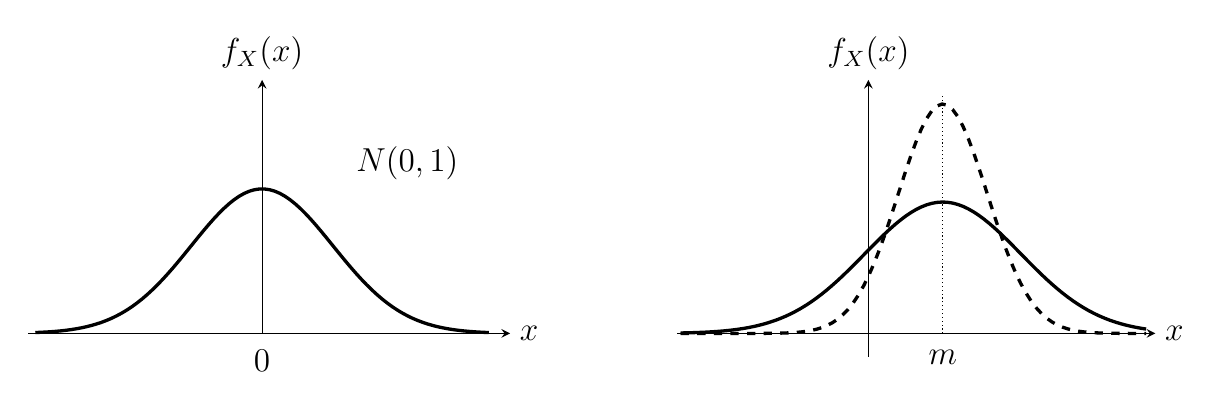
\begin{tikzpicture}[x=.9cm,y=4.6cm,>=stealth,font=\large]
  \draw[->] (-3.3,0)--(3.5,0) node[right] {$x$};
  \draw[->] (0,0)--(0,.7) node[above] {$f_X(x)$};
  \draw[very thick,domain=-3.2:3.2,samples=90]
    plot (\x,{exp(-(\x)^2/2)/sqrt(2*pi)});
  \node[below] at (0,-.02) {$0$};
  \node at (2.05,.47) {$N(0,1)$};
  \begin{scope}[xshift=7.7cm]
    \draw[->] (-2.7,0)--(4.05,0) node[right] {$x$};
    \draw[->] (0,-.065)--(0,.7) node[above] {$f_X(x)$};
    \draw[densely dotted] (1.05,0)--(1.05,.655);
    \draw[very thick,domain=-2.65:3.92,samples=90]
      plot (\x,{exp(-(\x-1.05)^2/(2*1.1^2))/(1.1*sqrt(2*pi))});
    \draw[very thick,dashed,domain=-2.65:3.92,samples=90]
      plot (\x,{exp(-(\x-1.05)^2/(2*.63^2))/(.63*sqrt(2*pi))});
    \node[below] at (1.05,-.02) {$m$};
  \end{scope}
\end{tikzpicture}
\end{document}
